\documentclass[UTF8]{ctexart}

\usepackage{subfiles}  

%下面的语句, 引入你的头部设置文件
\usepackage{C:/phpStorm_proj/02_myself_ID_EGO/+100_latex_all_math_sel/myPreamble} 
%必须是绝对路径,才能让各个tex在单独编译时使用到

\title{概率}


%---------------------------------


\begin{document}
	\tableofcontents % 生成目录
	\date{} % 若不写这句, 则默认也会渲染出日期, 所以我们要手动赋空值
	\maketitle  %这行代码, 让你前面的 title, author, date生效
	
	\part{基本概念}
	
	
	\section{排列 and 组合}
	
	\subsection{加法原理, 乘法原理}
	
	- 一件事, 只需``一步"就能完成. 但这一步中有几种不同的方案可供选择, 就用``加法"原理. \\	
	- 一件事, 要分成``几步骤"才能完成. 每一步, 又有几种不同的选择方案. 就用``乘法"原理. \\
	
	
	\begin{myEnvSample}
		上海汽车摇号, 成功率是 5\%. \\
		有灰产称: 能帮你将中签率从5\% 提高到 50\%, 只要三次就能保证你中签. \\
		→ 若成功 : 你车20的话, 他们就收你 10\% (即2万.) \\
		→ 若失败: 代理费全部返还你, 并再陪你 800元. \\
		问: 1.他们真的有内部资源吗? 2. 他们会亏还是赚? \\
		
		正常人, 摇号三次, 每月一次. 即三个月后中签的概率是多少呢? \\
		→ 错误的算法: $	0.05^3=0.000125	$. ← 这算的是``连续3个月, 每个月都能中奖的概率"! \\
		→ 正确的算法: 先算连续三个月, 每个月都没中奖的概率 ($=0.95^3=0.857375	$), 然后再1减去这个概率值 ($1-0.95^3=0.142625$). 这个结果, 就是``至少有一个月能中奖的概率", 即 14.2\%. \\
		
		现在, 我们就用 正常人三个月中的中一次奖的概率 14.2 \%, 来算算灰产的收益. \\
		灰产找来100人, 三个月后: \\
		→ 其中会有平均14\%个人中签. 每人收2万, 就是总收入 14×2=28万. \\
		→ 还有平均86个人没中签, 每人赔偿800元, 灰产支出 = 86×800 =68800元. \\
		→ 即灰产的总收入 = 收入28万 - 支出 6.88万 = 21.12万. \\
		显然, 灰产根本不需要什么内部资源, 直接普通人的中签概率, 就能在100人中, 净赚21.12万元. \\
		
		那么, 我们继续来算一下, 对于没中签的客户, 灰产要陪他们每人多少钱, 灰产才能不赚不亏呢?  即灰产能赚到的钱, 要全部赔出去. \\
		即: 
		\begin{align*}  % 支持每行编号. 若不需要编号, 就用 align*环境
&	280000\text{元总收入}=86\text{人}\cdot x\text{元}\\
& x=\frac{280000}{86}=3255.81\text{元/人}
		\end{align*} 
	
	所以如果你是客户, 要让灰产赔 3255元/人, 如果他们能够接受, 你才能相信他们的确可能有内部资源.
	
		
		
		
		

	\end{myEnvSample}
	
	
	
	
	
	
	
	
	
	
	
	
	\subsection{不重复排列 : $\text{P}_{\text{总数n}}^{\text{选出的数量m}}=\dfrac{\text{总数!}}{\text{(总数}-\text{选数)!}}		$}
	
	不重复排列: 就是从n个不同的元素中, 取出m个来排列, 排过的元素不放回, 没有下次排列资格了. 
	
	则, 所有可能的排列(Permutation)方案, 就是:	
	
	$
		\boxed{		\text{P}_{\text{总数n}}^{\text{选出的数量m}}=\text{n(n}-1\text{)(n}-2\text{)...(n}-\text{m}+1\text{)}=\dfrac{\text{n!}}{\text{(n}-\text{m)!}}=\dfrac{\text{总数!}}{\text{(总数}-\text{选数)!}} 
		}
	$
	
	\begin{myEnvSample}
		10人选5人上岸, 共有多少种选择?
		
		$
		\text{P}_{\text{总}10}^{\text{取}5}=\frac{\text{总!}}{\text{(总}-\text{选)!}}=\frac{10!}{\text{(}10-5\text{)!}}=30240
		$
	\end{myEnvSample}
	
	
	
	
	
	\subsection{全排列 : $\text{P}_{\text{总数n}}^{\text{n}}=\text{n!}	$ }
	
	全排列, 就是从n个里面, 取出全部n个来排列, 即所有的元素都参与了排列.
	
	$ \boxed{
	\text{P}_{\text{总数n}}^{\text{n}}=\text{n(n}-1\text{)(n}-2\text{)}...3\cdot 2\cdot 1=\text{n!}
	}
	$ \\
	
	例如:
	
	- $	\text{P}_{2}^{2}=2!=2	$ \\	
	- $ \text{P}_{1}^{1}=1!=1$ \\
	
		\begin{myEnvSample}
		一套书,共5本, 排在一起. 问: 自左向右, 或自右向左, 是按着1,2,3,4,5编号顺序的概率是?
		
		即 =$
		\dfrac{\text{顺序排是1种情况}+\text{倒序排是1种情况}}{\text{P}_{\text{总}5}^{\text{选}5}}=\dfrac{2}{\text{P}_{5}^{5}}=\dfrac{1}{60}=0.0166667
		$
	\end{myEnvSample} 


	
	- $0!=1$.  因为: 
	
	(1) 解释1: $\text{m!}=\text{m(m}-1\text{)!}$, 如 $10! =10 \cdot 9!$. 所以 $1! = 1 \cdot 0!$, 即得到 $0!=1$
	
	(2) 解释2: $P_{0}^{0}$ 就是从0个元素里面, 取出0个元素来排列. 这只有一种情况: 即 ``不选". 因为不存在任何元素, 所以没法选. 所以 $P_0^0=0!=1$ \\
	
	- $5^0 =1$ ← 因为 $5^0=5^{1-1}=\frac{5^1}{5^1}=1$ \\	
	- $0^0$ 无意义. ← 因为 $0^0=0^{1-1}=\frac{0^1}{0^1}$, 而分母不能为0, 所以该式子无意义.
	
	
	
	\subsection{重复排列}
	
	即: 排过队的元素, 可以拿回去, 重复参加后面的排队.  (但同一元素的位置交换 不能认为是不同排列。)
	
	重复排列: $\underset{\text{共取了m次的n}}{\underbrace{\text{n}\cdot \text{n}\cdot ...\cdot \text{n}}}=\text{n}^{\text{m}}	$ \\
	
		
	\subsection{``送利益"模型 (放球模型)}
	
	将$n_{benefit}$种利益, 随机投送给$N_{man}$个人 ($N_{man}\ge n_{benefit}$). 问: 每个人中, 最多只拿到1种利益的概率?
	
	→ 先看样本空间: 第1种利益, 有$N_{man}$个人的去向可供选择; 第2种利益, 同样如此, ... 所以, 根据``分步骤"法, 全部$n_{benefit}$种利益, 它们的所有去向, 就共有: $\underset{\text{共}n_{benefit}\text{个}}{\underbrace{N_{man}\cdot N_{man}\cdot ...\cdot N_{man}}}=N^n	$ 个.
	
	→ 再来看``每个人中, 最多只拿到1种利益": 第1个人,
	
	未完待续... 这里没看懂
	
	
	
%	\begin{myEnvSample}
%		假设每个人的生日, 在一年365天中的任何一天都是``等可能性"的, 即可能性均是 1/365. 问: \\
%		
%		(1) 随机取 n个人 ($n \leq 365$), 他们的生日各不相同 的概率是?
%		
%		那么第1个人, 可选的范围概率就是:  最自由, 在 365天里随便选1天. 即: $$
%		
%		
%		(2) n个人中, 至少两人生日相同的概率是?
%		
%		
%
%	\end{myEnvSample}
%	
	
	
	
	
	

	\subsection{组合 combination : $
		\text{C}_{\text{总}}^{\text{选}}=\frac{\text{总!}}{\text{选!}\left( \text{总}-\text{选!} \right)}	= C_{\text{总}}^{\text{总}-\text{选}}	$}
	
	组合: 是从n个不同元素中, 每次取出m个不同元素 ($0 \leq m \leq n$) , 合成一组, 而不需要管排队顺序, 就称为: 从n个元素中不重复地选取m个元素的一个组合. \\
	
	即: 有顺序, 就用排列; 无顺序, 就用组合. \\
	
	组合的公式是: 
	
$\boxed{
		\text{C}_{\text{总数}}^{\text{选数}}=\frac{\text{P}_{\text{总}}^{\text{选}}}{\text{选!}}=\frac{\text{总!}}{\text{选!}\left( \text{总}-\text{选!} \right)}	
}$

$\boxed{
		\text{C}_{\text{总}}^{\text{选}}=\text{C}_{\text{总}}^{\text{总}-\text{选}}	
}$ \\

上面第二个公式的意思是: 比如你有100人, 选其中10人上岸, 就相当于是选90人不上岸. 即: $\text{C}_{100}^{10}=\text{C}_{100}^{100-10}=\text{C}_{100}^{90}
$ \\

同理, 有 : $
\boxed{\text{C}_{\text{总}}^{0}=\text{C}_{\text{总}}^{\text{总}-0}=\text{C}_{\text{总}}^{\text{总}}
}$ \\
	
	
	\begin{myEnvSample}
		有共N人, 其中有w个女, 你任抽n人, 其中恰好有x个女人 ($x \leq w$) (记为事件A) 的概率是? 
		
		我们用``分步骤法"来做: 第一步, 先取x个女人. 第二步, 再取男人(数量就是= n-x). \\

$
\text{P(A)}=\dfrac{\text{取到x女}}{\text{从总N人中取n人}}=\dfrac{\overset{\text{第一步:先从全部女人里面,取x个女人}}{\overbrace{\text{C}_{\text{总w女}}^{\text{取x女}}}}\cdot \overset{\text{第二步:再从总男人里,取剩下的男人数量}}{\overbrace{\text{C}_{\text{总N人}-\text{总w女}=\text{总男人数}}^{\text{总取n人}-\text{x女}}}}}{\text{C}_{\text{总N人}}^{\text{取n人}}}
$ \\

上面这个公式, 其实就是``古典概型"里面的``超几何分布".
	\end{myEnvSample}
	
	
	
	\begin{myEnvSample}
		有共9球, 5白, 4黑. 任取3球, 问:
		
		(1) 是 2白1黑 的概率: 		
		$
		\text{P(2白1黑)}=\frac{\overset{\text{第一步:5白取}2}{\overbrace{\text{C}_{5}^{2}}}\cdot \overset{\text{第二步:4黑取}1}{\overbrace{\text{C}_{4}^{1}}}}{\underset{\text{总9取}3}{\underbrace{\text{C}_{9}^{3}}}}=0.47619
		$ \\
		
		(2) 取到的3球中, 无黑球 :		
		$
		\text{P(3白)}=\frac{\overset{5\text{白取}3}{\overbrace{\text{C}_{5}^{3}}}}{\underset{\text{总9取}3}{\underbrace{\text{C}_{9}^{3}}}}=0.119048
		$ \\
		
		(3) 取到的3球中, 颜色相同 : 		
		$
		\text{P(3球同色)}=\frac{\overset{5\text{白取}3}{\overbrace{\text{C}_{5}^{3}}}\overset{\text{或}}{\overbrace{+}}\overset{4\text{黑取}3}{\overbrace{\text{C}_{4}^{3}}}}{\underset{\text{总9取}3}{\underbrace{\text{C}_{9}^{3}}}}=0.166667
		$
		
		或, 也可用第二种思路来解:  		
		\begin{align*}  % 支持每行编号. 若不需要编号, 就用 align*环境
	&\text{P(3球同色)}=1-\text{P(3球存在不同色)}\\
&=1-\frac{1\text{白2黑,\ 或2白1黑}}{9\text{取}3}\\
&=1-\frac{\overset{5\text{白取}1; }{\overbrace{\text{C}_{5}^{1}}}\overset{4\text{黑取}2}{\overbrace{\text{C}_{4}^{2}}}\overset{\text{或}}{\overbrace{+}}\overset{5\text{白取}2; }{\overbrace{\text{C}_{5}^{2}}}\overset{4\text{黑取}1}{\overbrace{\text{C}_{4}^{1}}}}{\text{C}_{9}^{3}}\\
&=0.166667
		\end{align*}

	\end{myEnvSample}
	
	
	

	
	\section{交集 $\cap$ , 与 并集 $\cup$}
	
	A, B, C 是 试验E 的随机事件. 则表示法是:
	
	- A发生 : $A$ \\
	
	下面, 加法即表示``或" :
	
	- A, B, C 恰有一个发生 : $A\overline{B}\overline{C}+\overline{A}B\overline{C}+\overline{A}\overline{B}C$
	
	- A, B, C 至少一个发生(即 >=1) : A+B+C 或 $A{\cup}B{\cup}C$ ← 即3选1, 还有两个发不发生, 不用管, 随意, 都行.
	
	- A, B, C 至多一个发生(即 <=1) : $\underset{3\text{选}1}{\underbrace{A\overline{B}\overline{C}+\overline{A}B\overline{C}+\overline{A}\overline{B}C}}+\underset{3\text{选}0}{\underbrace{\overline{A}\overline{B}\overline{C}}}		$
		
	- 恰有两个发生: $AB \overline{C} + A \overline{B} C + \overline{A} BC $
	
	- 至少两个发生(即,>=2 ) : $\underset{3\text{选}2}{\underbrace{AB\overline{C}+A\overline{B}C+\overline{A}BC}}+\underset{3\text{选}3}{\underbrace{ABC}}+\underset{3\text{选2,\ 还有一个发不发生不用管,随意}}{\underbrace{AB+BC+AC}}	$	\\
		
		

	下面, 乘法即表示``同时" :	
	
	- 只有A发生 : $A\overline{B}\overline{C}$	

	- A, B, C 同时发生 : ABC  \\
	
\begin{myEnvSample}
	一次射击试验, 整个流程是打三枪, 用 $A_i, (i=1,2,3)$ 来表示``在第i次时击中了目标".
	
	记住: 加法(+) 代表``或,并 $\cup$"; 乘法代表``交$\cap$".
	
	- $A_1+A_2$ : 表示第一次击中了, 或第二次击中了. 即前两次至少击中一次.
	
	- $	\overline{A_2}	$ : 表示第二次没击中.
	
	- $	A_1+A_2+A_3	$ : 表示仅第一次击中, 或仅第二次击中, 或仅第三次击中.
	
	- $	A_1A_2A_3	$ : 表示三次全中.
	
	- $	A_2\overline{A_3} = A_2 - A_3	$ : 表示第二次击中, 并且第三次失败.
	
	- $	\overline{A_1}\cap \overline{A_3}=\overline{A_1+A_3}$ : 表示第一次没中, 并且第三次也没中.
	
	- $	\overline{A_1}+\overline{A_3}	$ : 表示第一次没中, 或第三次没中.


\end{myEnvSample}



\section{频率}

做n次试验, A事件发生了m次, 我们就把 $\dfrac{A\text{事件发生的次数}m}{\text{共}n\text{次试验}}$ 叫做``频率". 记作$\omega _n\left( A \right) $.

比如丢硬币, 丢10次, 丢100次, 丢1000次, 每次的``频率"可能都不一样, 比如结果是 $\frac{7}{10},\frac{55}{100},\frac{508}{1000} $. 所以这就是``频率"和``概率"的区别.

但你可以发现, 随着试验次数n的增大, A事件的``频率"的值, 会接近与``概率"的值. 即: $ \lim_{n→0}\omega _n\left( A \right)  \to P $


\section{频率的性质:}

规范性: 

- $\omega _n\left( \varOmega \right) =1$ ← 做n次试验, 里面``必然事件"发生的频率, 是1.  
既然是``必然事件Ω", 它肯定会发生, 所以频率肯定是1.


- $\omega _n\left( \varPhi \right) =0$ ← 做n次试验, 里面``不可能事件"发生的频率, 是0. \\



可加性: 


比如做1000次试验, 即$ \varOmega_{1000}$, 则有: 

$\omega _{1000}\left( A_1+A_2 \right) =\underset{1000\text{次试验中,}A1\text{事件发生的频率}}{\underbrace{\omega _{1000}\left( A_1 \right) }}+\underset{1000\text{次试验中,}A2\text{事件发生的频率}}{\underbrace{\omega _{1000}\left( A_2 \right) }}$ \\

即: ``和的频率", 就等于``频率的和".

$
\boxed{
\underset{\text{做}n\text{次试验,里面有}m\text{个事件发生了的频率}}{\underbrace{\underset{\text{做}n\text{次试验}}{\underbrace{\omega _n}}\underset{\text{里面有}m\text{个事件}}{\underbrace{\left( A_1+A_2+...+A_m \right) }}}}=\omega _n\left( A_1 \right) +\omega _n\left( A_2 \right) +...+\omega _n\left( A_m \right) 
}
$



	
\section{公理化}
	
	\subsection{$P(A) + P(\overline{A}) = 1$}
	
	\subsection{对于``完备事件组"中的所有事件来说: $P(A_1) + P(A_2) + ... +  P(A_n) =  P(\Omega) = 1$}
	
	完备事件组 collectively exhaustive events 就是: 如果事件 B1, B2, B3, ...  Bn 满足:
	
	1. 它们两两互不相容(即两两的交集=空集),
	
	2. 其``和"为全集 Ω. 	
	
	换言之, 若n个事件两两互斥, 且这n个事件的``并"是 Ω,则称这n个事件为``完备事件组". \\
	
	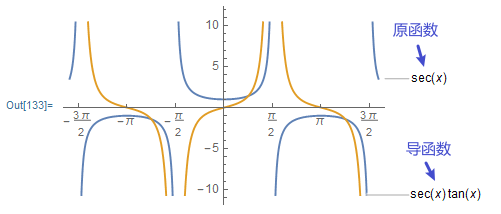
\includegraphics[width=0.6\textwidth]{/0069.png}
	
	
	\begin{myEnvSample}
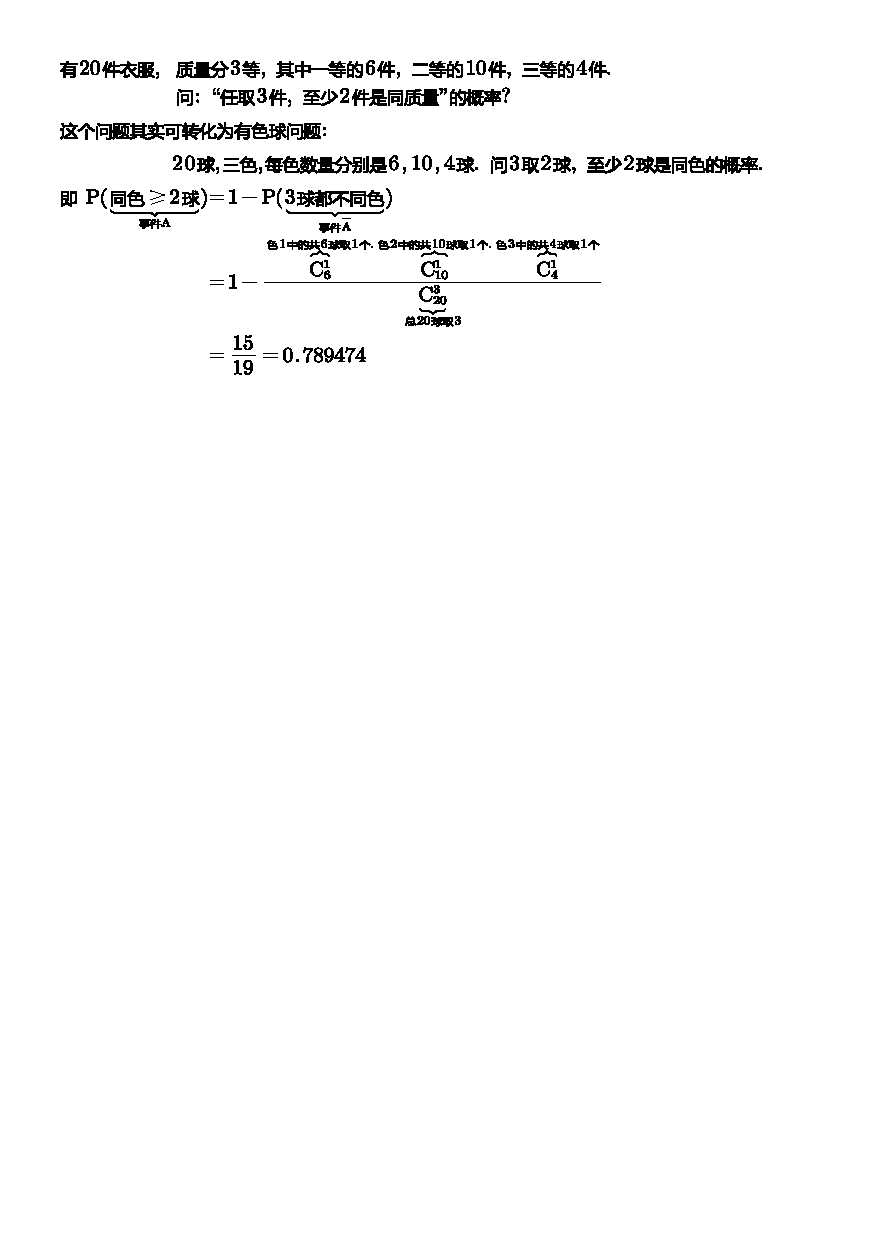
\includegraphics[width=0.9\textwidth]{/0076.pdf} \\

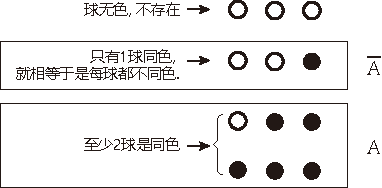
\includegraphics[width=0.5\textwidth]{/0077.pdf}
	\end{myEnvSample}
	
	
	\begin{myEnvSample}
	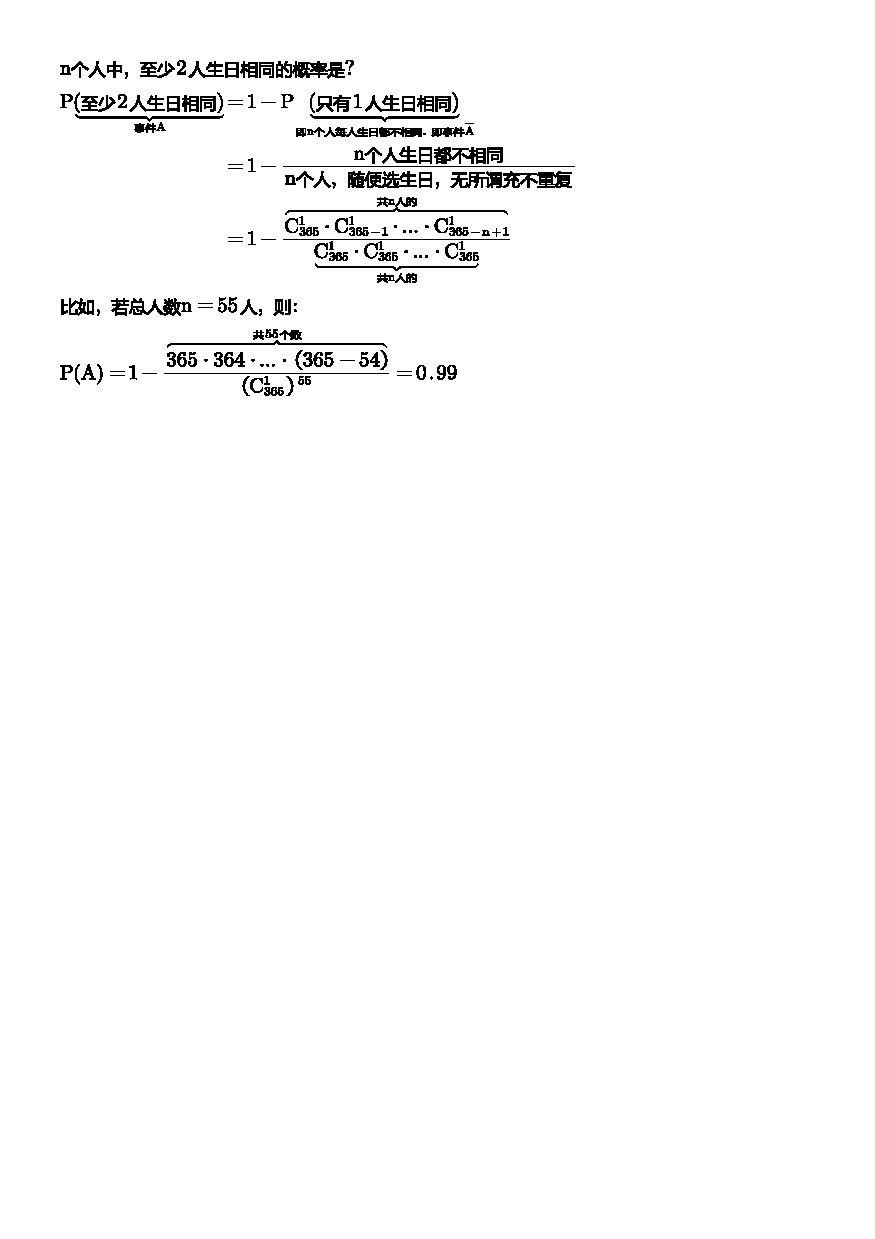
\includegraphics[width=0.65\textwidth]{/0079.pdf} \\
		
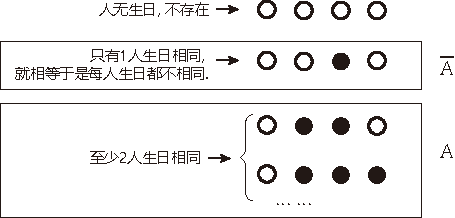
\includegraphics[width=0.6\textwidth]{/0078.pdf} 
	\end{myEnvSample}
	
	
	
	\subsection{$P(A-B) = P(A) - P(AB)$}	
		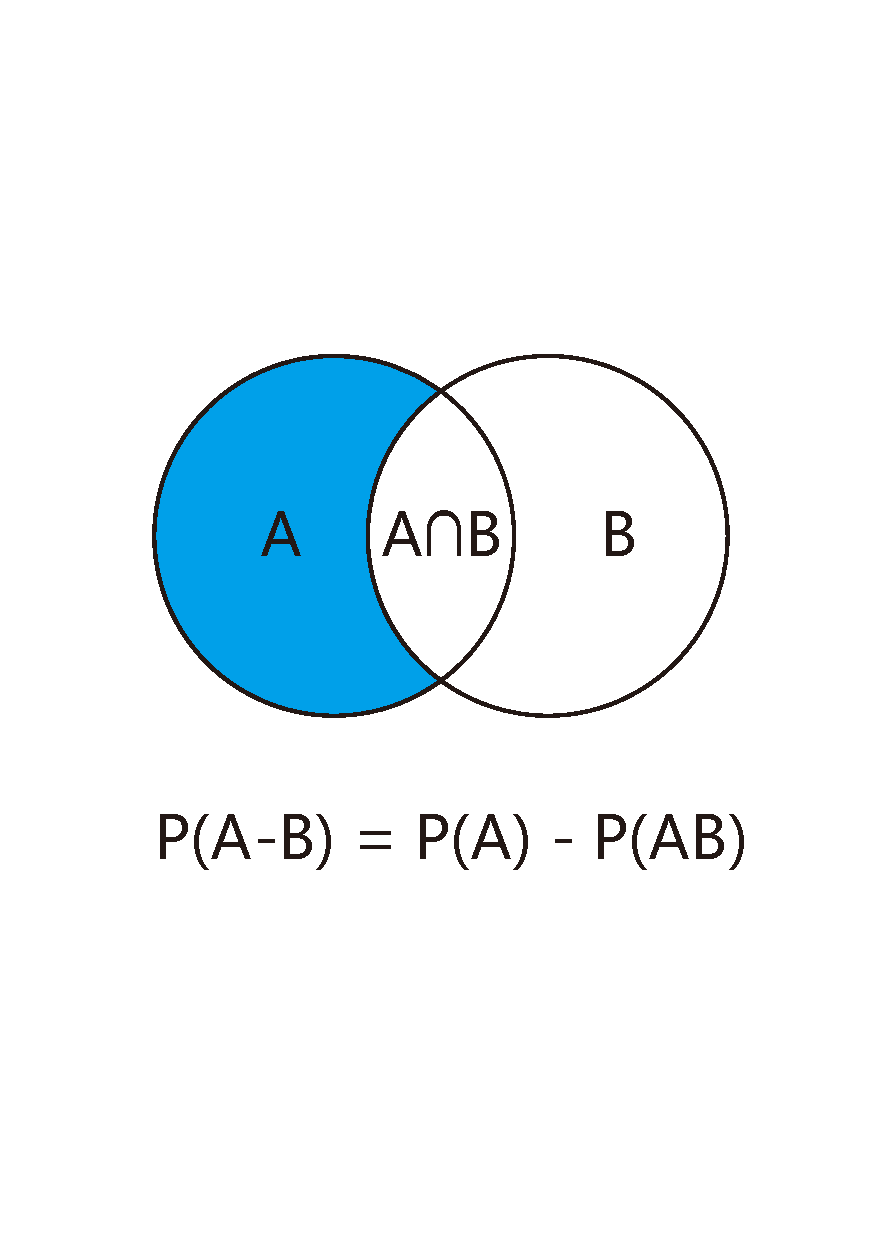
\includegraphics[width=0.2\textwidth]{/0070.pdf}
		
	
	\subsection{若A包含着B, 则有: $ P(A-B) = P(A) - P(B)$, 且 $P(A) >= P(B) $}
	
	
	\subsection{加法公式: $ P(A+B) = P(A) + P(B) - P(AB)$}	
	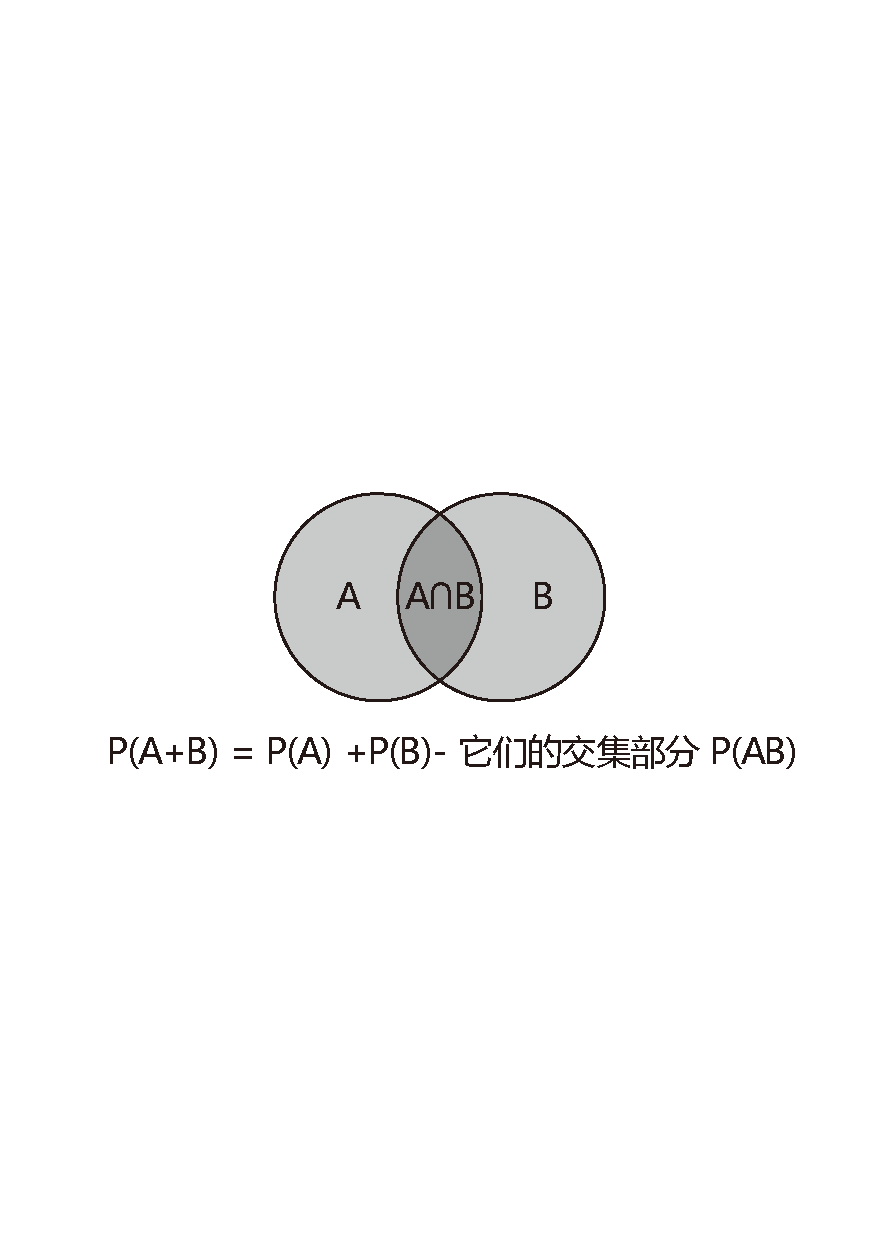
\includegraphics[width=0.4\textwidth]{/0071.pdf} \\
	
	\begin{myEnvSample}
		A事件的概率是0.4, 即 P(A)=0.4; 
		
		P(B)=0.3; 
		
		且P(A+B)=0.6, ← 说明A与B有交集部分存在. 否则, 如果A与B是不相容的话, 它们和的概率, 应该是 0.4+0.3=0.7.
		
		所以它们的交集 P(AB) 就是=0.1 : 
		
		$
		\underset{0.6}{\underbrace{P\left( A+B \right) }}=\underset{0.4}{\underbrace{P\left( A \right) }}-\underset{0.3}{\underbrace{P\left( B \right) }}-\underset{=0.1}{\underbrace{P\left( AB \right) }}
		$ \\
		
		求$P\left( A\overline{B} \right)$, 即求$A \cap B\text{逆}$ 的概率: 
		
$
P\left( A\cap \overline{B} \right) =P\left( A-B \right) =\underset{=0.4}{\underbrace{P\left( A \right) }}-\underset{=0.1}{\underbrace{P\left( AB \right) }}=0.3
$ \\

	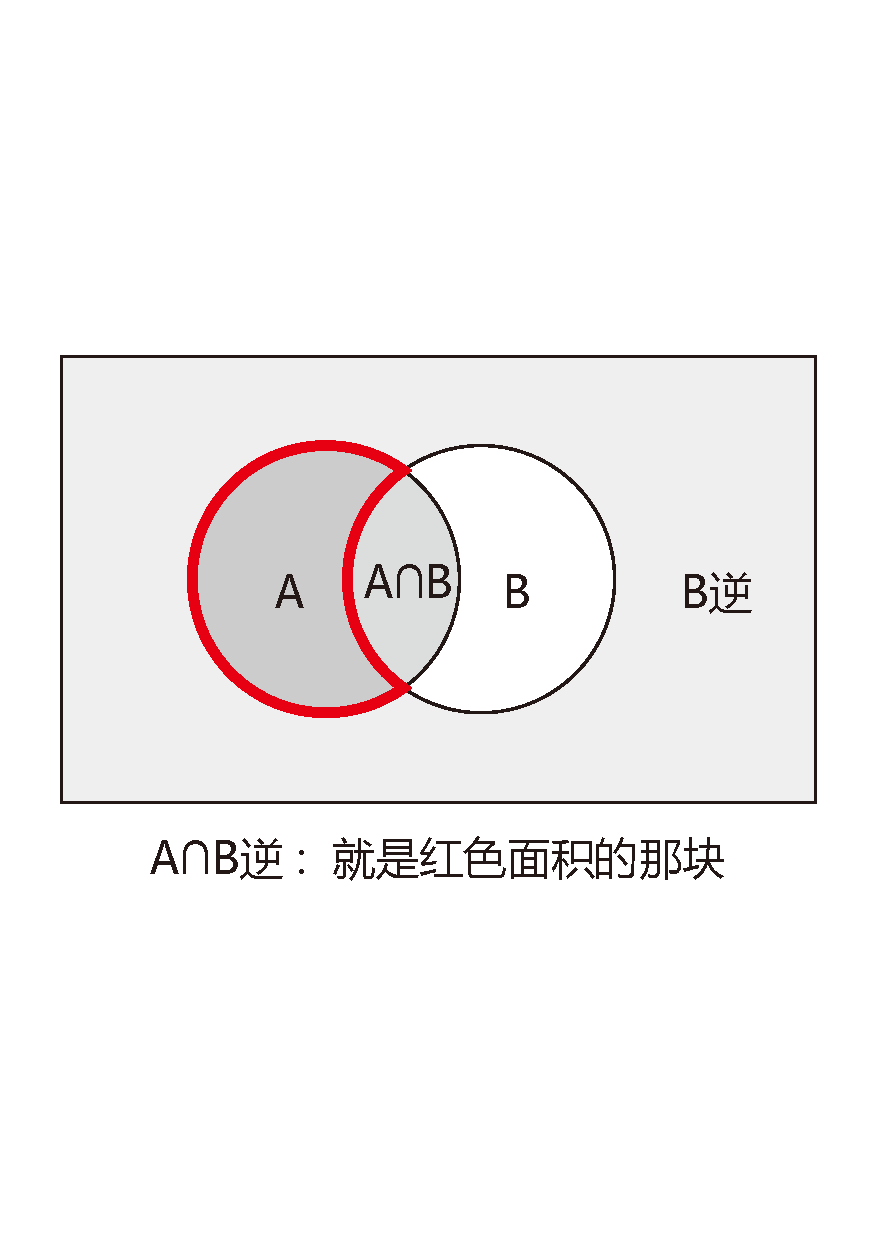
\includegraphics[width=0.35\textwidth]{/0073.pdf}
	
		\end{myEnvSample}
	
	
	
	
	
	\subsection{加法公式: $ P(A+B+C) = P(A) + P(B)  +  P(C) - P(AB) - P(AC) -  P(BC) +  P(ABC)$}
	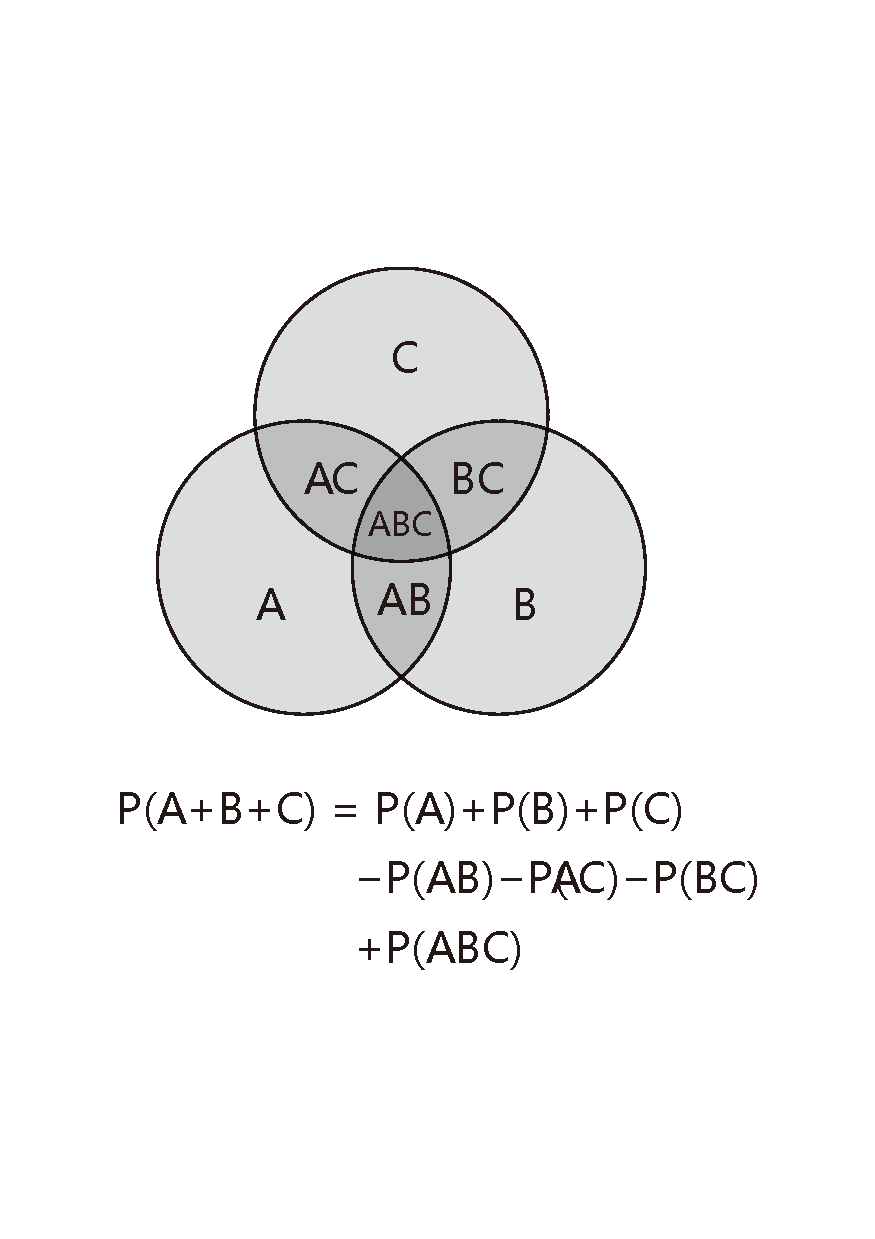
\includegraphics[width=0.3\textwidth]{/0072.pdf}	
	
	说明: 
	\begin{align*}  % 支持每行编号. 若不需要编号, 就用 align*环境
	& P\left( A+B+C \right) \\
&=\underset{\text{这里,}ABC\text{交集部分,被加了3次}}{\underbrace{P\left( A \right) +P\left( B \right) +P\left( C \right) }}\underset{\text{这里,}ABC\text{交集部分,又减了3次}}{\underbrace{-P\left( AB \right) -P\left( AC \right) -P\left( BC \right) }}+\underset{\text{所以最后,我们还要把镂空的}ABC\text{交集部分,加上一份上去}}{\underbrace{P\left( ABC \right) }}
	\end{align*}

	
	\begin{myEnvSample}
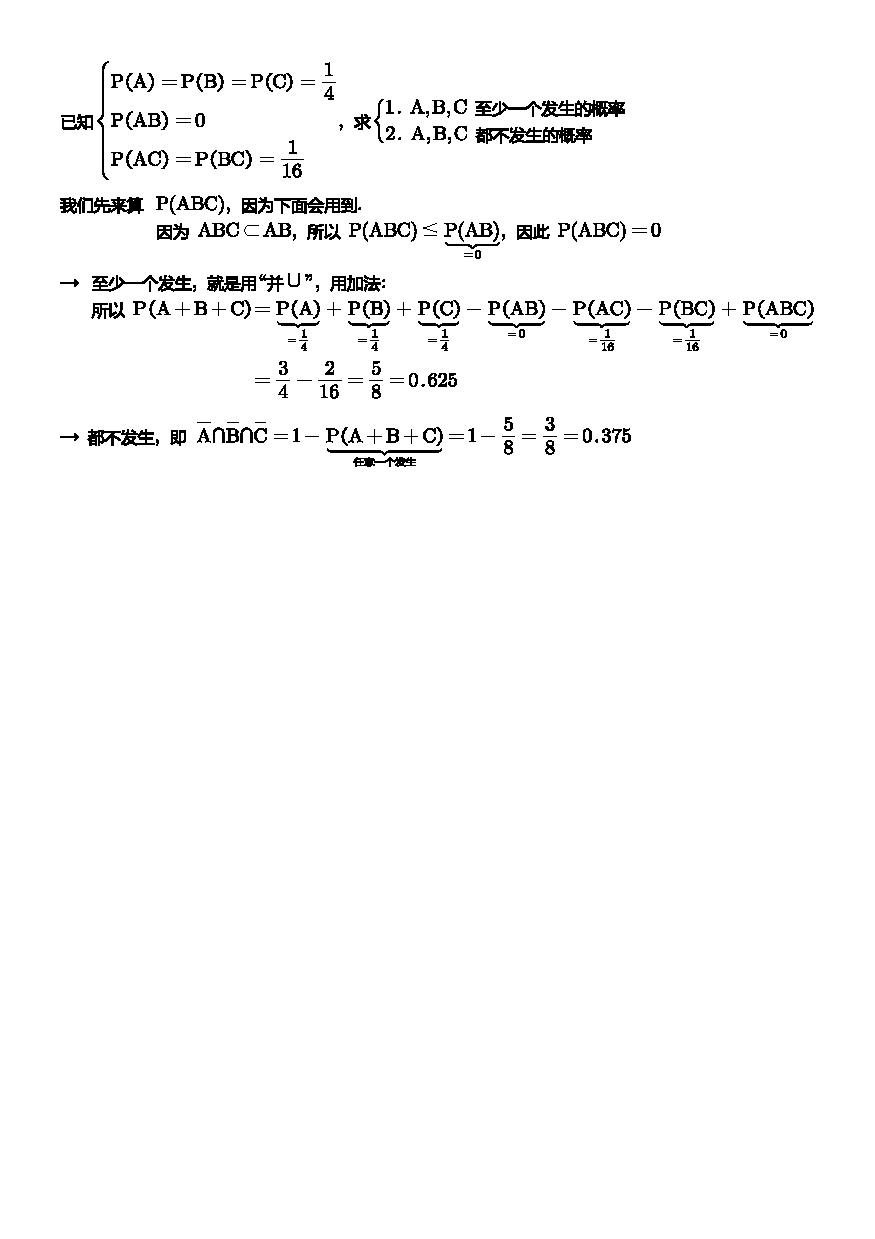
\includegraphics[width=1\textwidth]{/0074.pdf}
	\end{myEnvSample} 
	
	\begin{myEnvSample}
	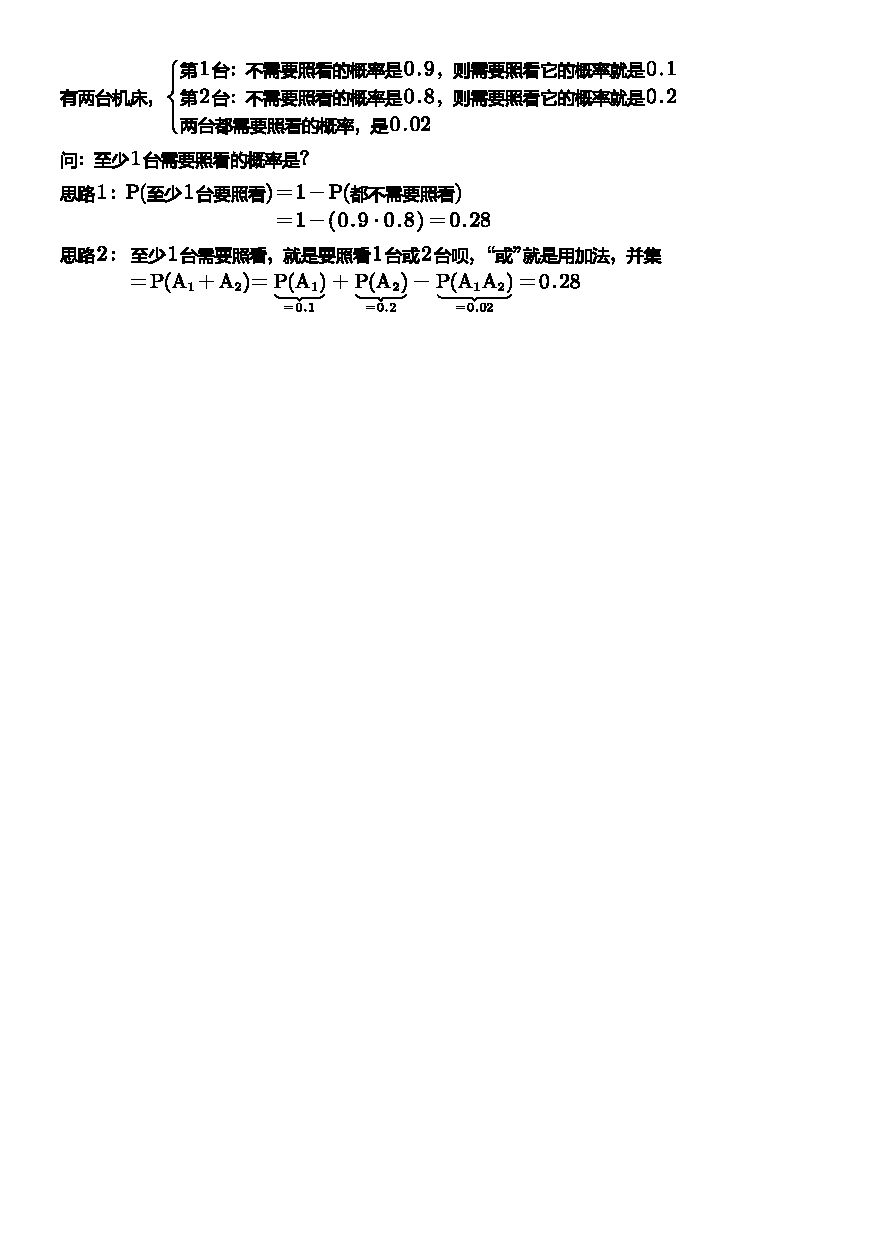
\includegraphics[width=0.82\textwidth]{/0075.pdf}
\end{myEnvSample}


~\\
\hrule
~\\


\section{古典概型 : $\text{P(A)}=\dfrac{\text{A中包含的``基本事件"有多少个}}{\text{S中``基本事件"的总数}}$}


满足这些条件的, 就属于``古典概率  classical models of probability 模型":

- 样本点是有限的

- 所有样本点出现的可能性, 是相同的. 即``等可能性". \\


古典概型模型:

事件$\text{A}=\{\text{e}_{\text{i}_1},\text{e}_{\text{i}_2},...,\text{e}_{\text{i}_{\text{k}}}\}$ 发生的概率为:

$
\text{P(A)}=\dfrac{\text{k}}{\text{n}}=\dfrac{\text{A中包含的``基本事件"有多少个}}{\text{S中``基本事件"的总数}}
$ \\


古典概率模型的性质:

- $0 <= P(A) <= 1$

- $P(\Omega)=1, \quad  P(\Phi)=0$

- 有限可加 : $ A_1, A_2, ... A_n$ 是互不相容的. 即 $P(A_1 +A_2 + ...+ A_n)= P(A_1) +  P(A_2)  + P(A_n)$ \\

古典概率模型: 

- 其优点是: 可以直接套公式来算. 

- 但其缺点是: 

(1) 其结果必须是``有限个"的结果 (如, 掷骰子, 结果就是6个基本事件, 而不是无限个事件.) 

(2)其结果, 必须是``等可能性".


	

\begin{myEnvSample}
	有 a个白, b个黑, 问: 从中连续取出 m个球 (连续取, 就是不放回的意思了) ($1 \leq m \leq a+b$), 第m个 是白球的概率= ? \\
	
	思路1 : 其实我们只要考虑 第 m 个位置的这一个球的情况就行了, 其他位置的球,随便它们什么颜色, 我们不用考虑的.
	
	$\text{P}\left( \text{第m位置是白球} \right) =\frac{\text{在第m个位置上,\ 从a个白球里取1个放上去.\ 剩下数量的其他位置上,\ 依然做全排列}}{\text{所有球的全排列}}
	$ \\
	
	即 $	\text{P}\left( \text{第m位置是白球} \right) =\frac{\overset{\text{第一步,\ 先取1个白球,占位放在第m个位置上.}}{\overbrace{\text{C}_{\text{总a白}}^{\text{取}1}}}\cdot \overset{\text{第二步:剩下的所有球,\ 依然做全排列}}{\overbrace{\text{C}_{\text{总a白}+\text{总b黑}-1}^{\text{总a白}+\text{总b黑}-1}}}}{\text{P}_{\text{总a白}+\text{总b黑}}^{\text{总a白}+\text{总b黑}}}
	$ \\
	
	
	思路2 : 或者我们也只需考虑前m个数量的球就行了, 后面其他的球, 爱怎样颜色怎样颜色, 不用我们考虑.
	
	$	\text{P}\left( \text{第m位置是白球} \right) =\frac{\overset{\text{第一步,\ 先取1个白球,占位放在第m个位置上}}{\overbrace{\text{C}_{\text{总a白}}^{\text{取}1}}}\cdot \overset{\text{第二步:m个数中的剩下的所有球,\ 依然做全排列}}{\overbrace{\text{C}_{\text{总a白}+\text{总b黑}-1}^{\text{m}-1}}}}{\underset{\text{m个球的全排列}}{\underbrace{\text{P}_{\text{总a白}+\text{总b黑}}^{\text{m}}}}}
	$ \\
	\\
	
	其实你有没有发现? ``在第m个位置上出现白球" 这个``m索引位置", 其实是个障眼法. 白球出现在任何其他位置, 它出现在第1个位置, 第10个位置, 最后一个位置, 对我们的计算结果没有任何影响.  因为不管白球出现在第几个位置上, 它出现的概率都是相同的, 因为是古典概率嘛! 所以, ``位置为几"其实不重要. \\
	
	所以, 我们就有了第三种思路: 我们就把这个白球, 让它直接出现在第1个位置就好了:
	
	$	\text{P}\left( \text{第1个位置是白球} \right) =\frac{\overset{\text{(在第1个位置上,)\ 从白球里,\ 取1个\ 的取法数量}}{\overbrace{\text{C}_{\text{总a白}}^{1}}}}{\underset{\text{(在第1个位置上,)\ 从总数里,\ 取1个\ 的取法数量}}{\underbrace{\text{C}_{\text{总a白}+\text{总b黑}}^{1}}}}=\frac{\text{a}}{\text{a}+\text{b}}
	$		
\end{myEnvSample}




~\\
\hrule
~\\


\section{几何概型}


几何概型 geometric models of probability, 即这类概率问题, 能够转换成用``几何问题"来求解.

\begin{myEnvSample}
	有甲乙两人, 相约在 6-7点见面 (其实这个具体的时间点也是个障眼法, 只要在1个小时的区间就行). 先到者, 最多等对方15分钟, 然后就离开了.
	
	甲乙两人, 在这1小时内的任意时刻, 都可能到达.
	
	问, 他们能相见的概率是多少? \\
	
	我们令 
	
	- 事件A : 表示两人见到了面 \\
	- x : 表示甲到达的时间点 \\
	- y : 表示乙到达的时间点 \\
	
	他们要能见到面, 即 $|y-x| \leq 15$分钟. 那么这就有两种可能性: \\
	-  甲先到. 即 $x \leq y$ (甲来到的时间点x, 比乙来到的时间点y 要小 (早)), 即 $ y-x \leq 15$ \\
	-  乙先到. 即 $y \leq x$, 即 $ x-y \leq 15$ \\	
	
	这两组不等式, 能用函数图形来表示出来, 如下图. x和y轴上的60, 分别代表两人的1小时区间(60分钟) . 中间的交集区域, 就是两人可以见到面的时间段. \\
	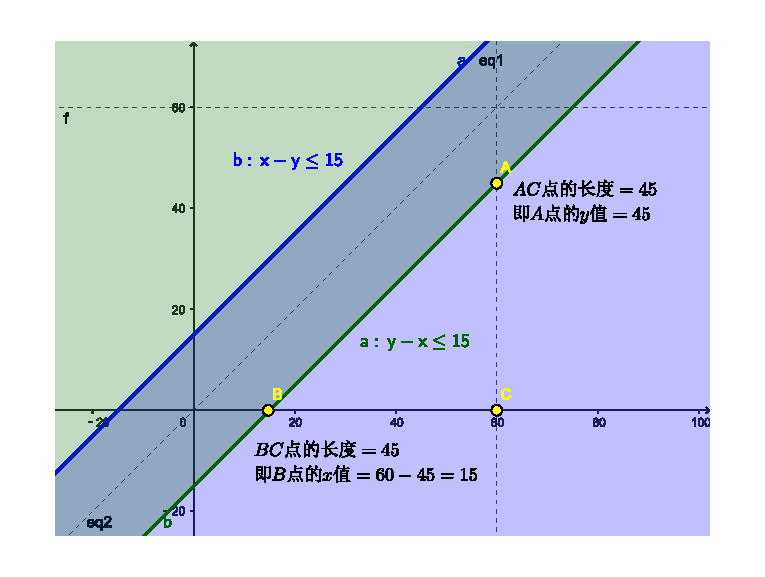
\includegraphics[width=0.9\textwidth]{/0083.pdf} \\
	
	显然, 这就是求几何面积的问题. \\
	
	即: $
	\text{P}\left( \text{A} \right) =\frac{60\cdot 60-\overset{\text{上面的``边长为45"的三角形的面积}}{\overbrace{\frac{45\cdot 45}{2}}}-\overset{\text{下面的``边长为45"的三角形的面积}}{\overbrace{\frac{45\cdot 45}{2}}}}{\underset{\text{即``边长为60分钟"的矩形}}{\underbrace{60\cdot 60}}}=0.4375
	$
\end{myEnvSample} 



\newpage

\begin{myEnvSample}
	(法国)布丰(1707-1788) 投针 Buffon's needle problem. \\
说: 有两条平行的直线, 相聚为 D(distance), 距离单位不重要. 你哪一个针 (长度为 L (length), $L<D$), 随机地投向针. 问: 针与那两条平行直线 相交的概率是? \\

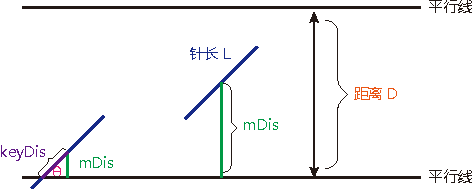
\includegraphics[width=0.6\textwidth]{/0086.pdf} \\
\end{myEnvSample} 


	思路: 针投上去后的位置状态, 是由两个参数决定的: \\
(1) 针的中点, 距离``最近那根直线"的最短距离. ← 该距离用变量 mDis (midpoint distance)来表示. \\
(2) 针倾斜的位置, 与直线的夹角. ← 我们用变量 $\theta$ 来表示.  \\
用上面这两个变量, 我们能分别作为 x轴(表示 $\theta$ 变量) 和 y轴(表示 mDis变量), 来画出函数图像. \\
		
	针投出后, 所有可能的状态, 其全集就是: \\
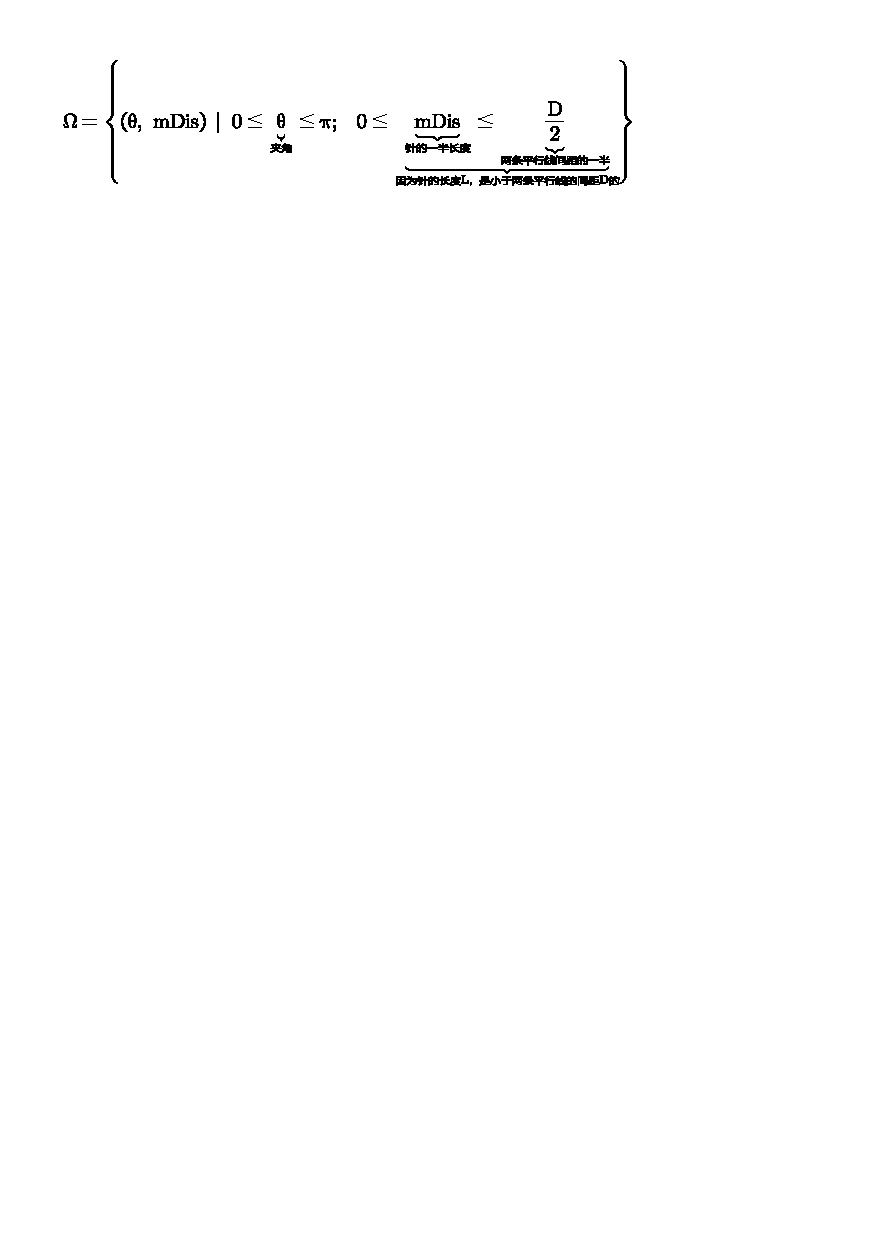
\includegraphics[width=0.8\textwidth]{/0084.pdf} \\
			
	那么, 什么状态下, ``针"就与``直线"相交了呢? -- 当``从针的中点(沿着针的身体走)到直线"的距离 (下面用变量 keyDis (key distance) 来表示这个距离) $\leq$ 针的一半长度时. 它们就相交了. 否则, 它们就不想交. \\
	即, 就有: \\	
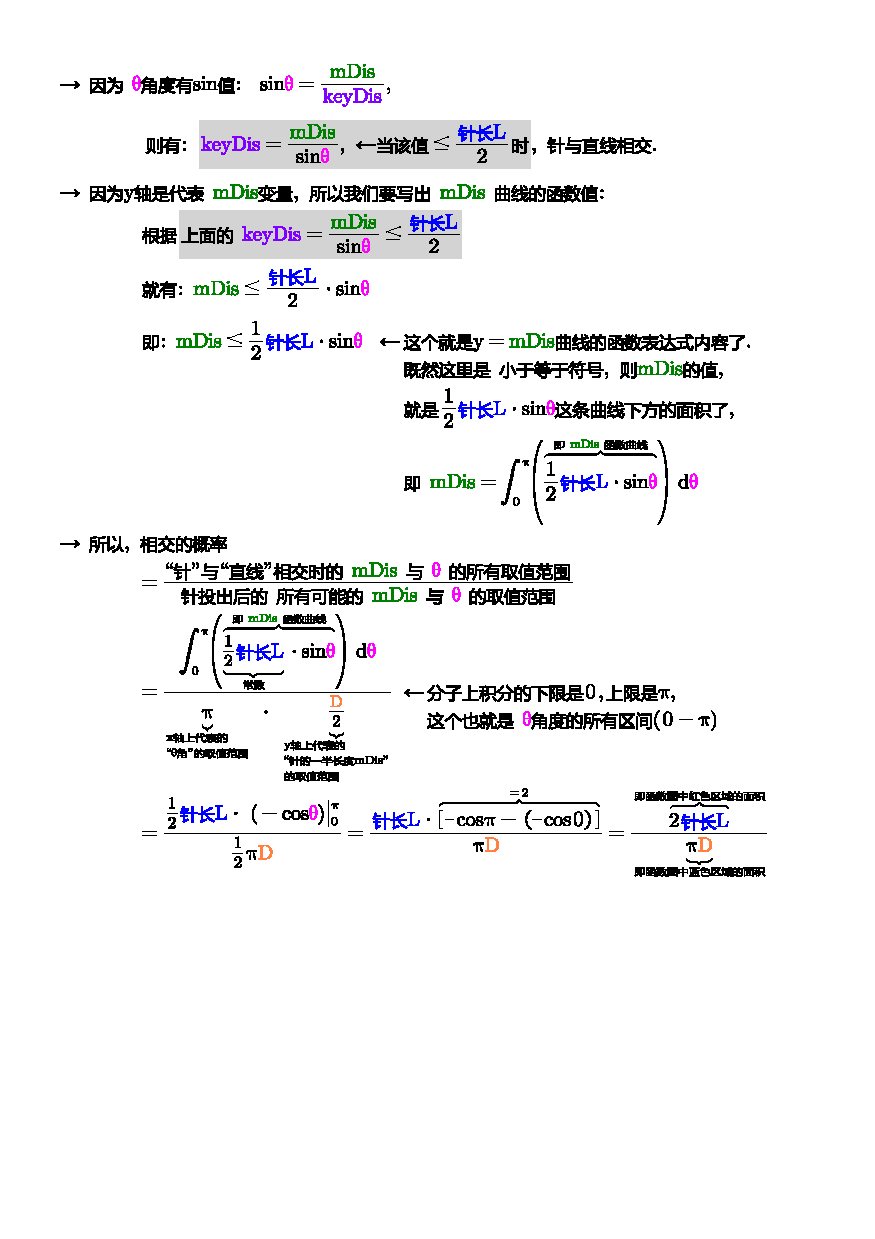
\includegraphics[width=0.97\textwidth]{/0085.pdf}

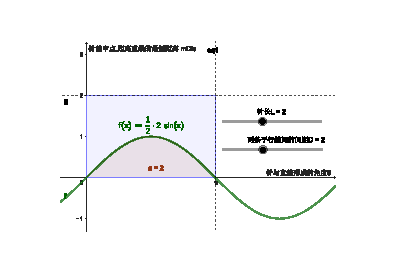
\includegraphics[width=0.8\textwidth]{/0087.pdf}




\subsection{``古典概率模型"和``几何概率模型"的区别}

- 古典概率模型 : \\
具有 ``有限可加性" (finite additivity): 是指``有限个"两两互不相容事件的``和事件"的概率, 等于``每个事件概率"的和. \\
即: $
\underset{\text{的概率}}{\underbrace{\text{P}\underset{\text{和}}{\underbrace{\left( \text{∪}_{\text{i}=1}^{\text{n}}\text{A}_{\text{i}} \right) }}}}=\underset{\text{的和}}{\underbrace{\sum_{\text{i}=1}^{\text{n}}{\underset{\text{概率}}{\underbrace{\text{P}\left( \text{A}_{\text{i}} \right) }}}}}
$ \\
\\

- 几何概率模型 : \\
具有``完全可加性":  即先求和, 再求概率, 等于 先求每个事件概率, 再求和. \\
即: $
\underset{\text{的概率}}{\underbrace{\text{P}\underset{\text{和}}{\underbrace{\left( \text{∪}_{\text{i}=1}^{\infty}\text{A}_{\text{i}} \right) }}}}=\underset{\text{的和}}{\underbrace{\sum_{\text{i}=1}^{\infty}{\underset{\text{概率}}{\underbrace{\text{P}\left( \text{A}_{\text{i}} \right) }}}}}
$ \\

注意两者的区别: 一个是``有限(到n)"的加,  一个是``无限(到∞)"的加.


	
\end{document}